\hypertarget{group__Provision}{\section{Provision}
\label{group__Provision}\index{Provision@{Provision}}
}


\mbox{[}Ordering 200\mbox{]} Provisioning stage  


Collaboration diagram for Provision\-:
\nopagebreak
\begin{figure}[H]
\begin{center}
\leavevmode
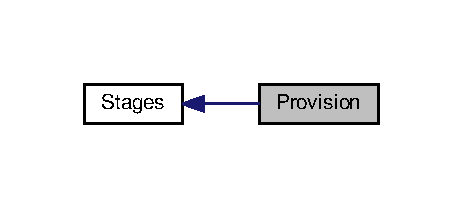
\includegraphics[width=222pt]{group__Provision}
\end{center}
\end{figure}
\mbox{[}Ordering 200\mbox{]} Provisioning stage \hypertarget{group__Provision_WWulf3}{}\subsection{W\-Wulf3}\label{group__Provision_WWulf3}
Plugin for provisioning nodes using the Warewulf v3 image manager 
\begin{DoxyParams}{Parameters}
{\em target} & List of remote host names or L\-A\-N interfaces to be provisioned \\
\hline
{\em image} & Name of image to be instantiated \\
\hline
{\em bootstrap} & Name of bootstrap to be used \\
\hline
{\em controller} & List of I\-P addresses of remote node controllers/\-B\-M\-Cs \\
\hline
{\em username} & Remote controller username \\
\hline
{\em password} & Remote controller password \\
\hline
{\em pwfile} & File containing remote controller password \\
\hline
{\em sudo} & Use sudo to execute privileged commands \\
\hline
{\em allocate\-\_\-cmd} & Command to use for allocating nodes from the resource manager \\
\hline
{\em deallocate\-\_\-cmd} & Command to use for deallocating nodes from the resource manager \\
\hline
\end{DoxyParams}
